
\documentclass[border=10pt, 12pt]{standalone}
\usepackage[svgnames]{xcolor}
\usepackage{amsmath}
\usepackage{pgfplots}
\pgfplotsset{compat=newest}
\usepackage[sfdefault]{FiraSans}
\usepackage{FiraMono}
\renewcommand*\familydefault{\sfdefault}
\begin{document}
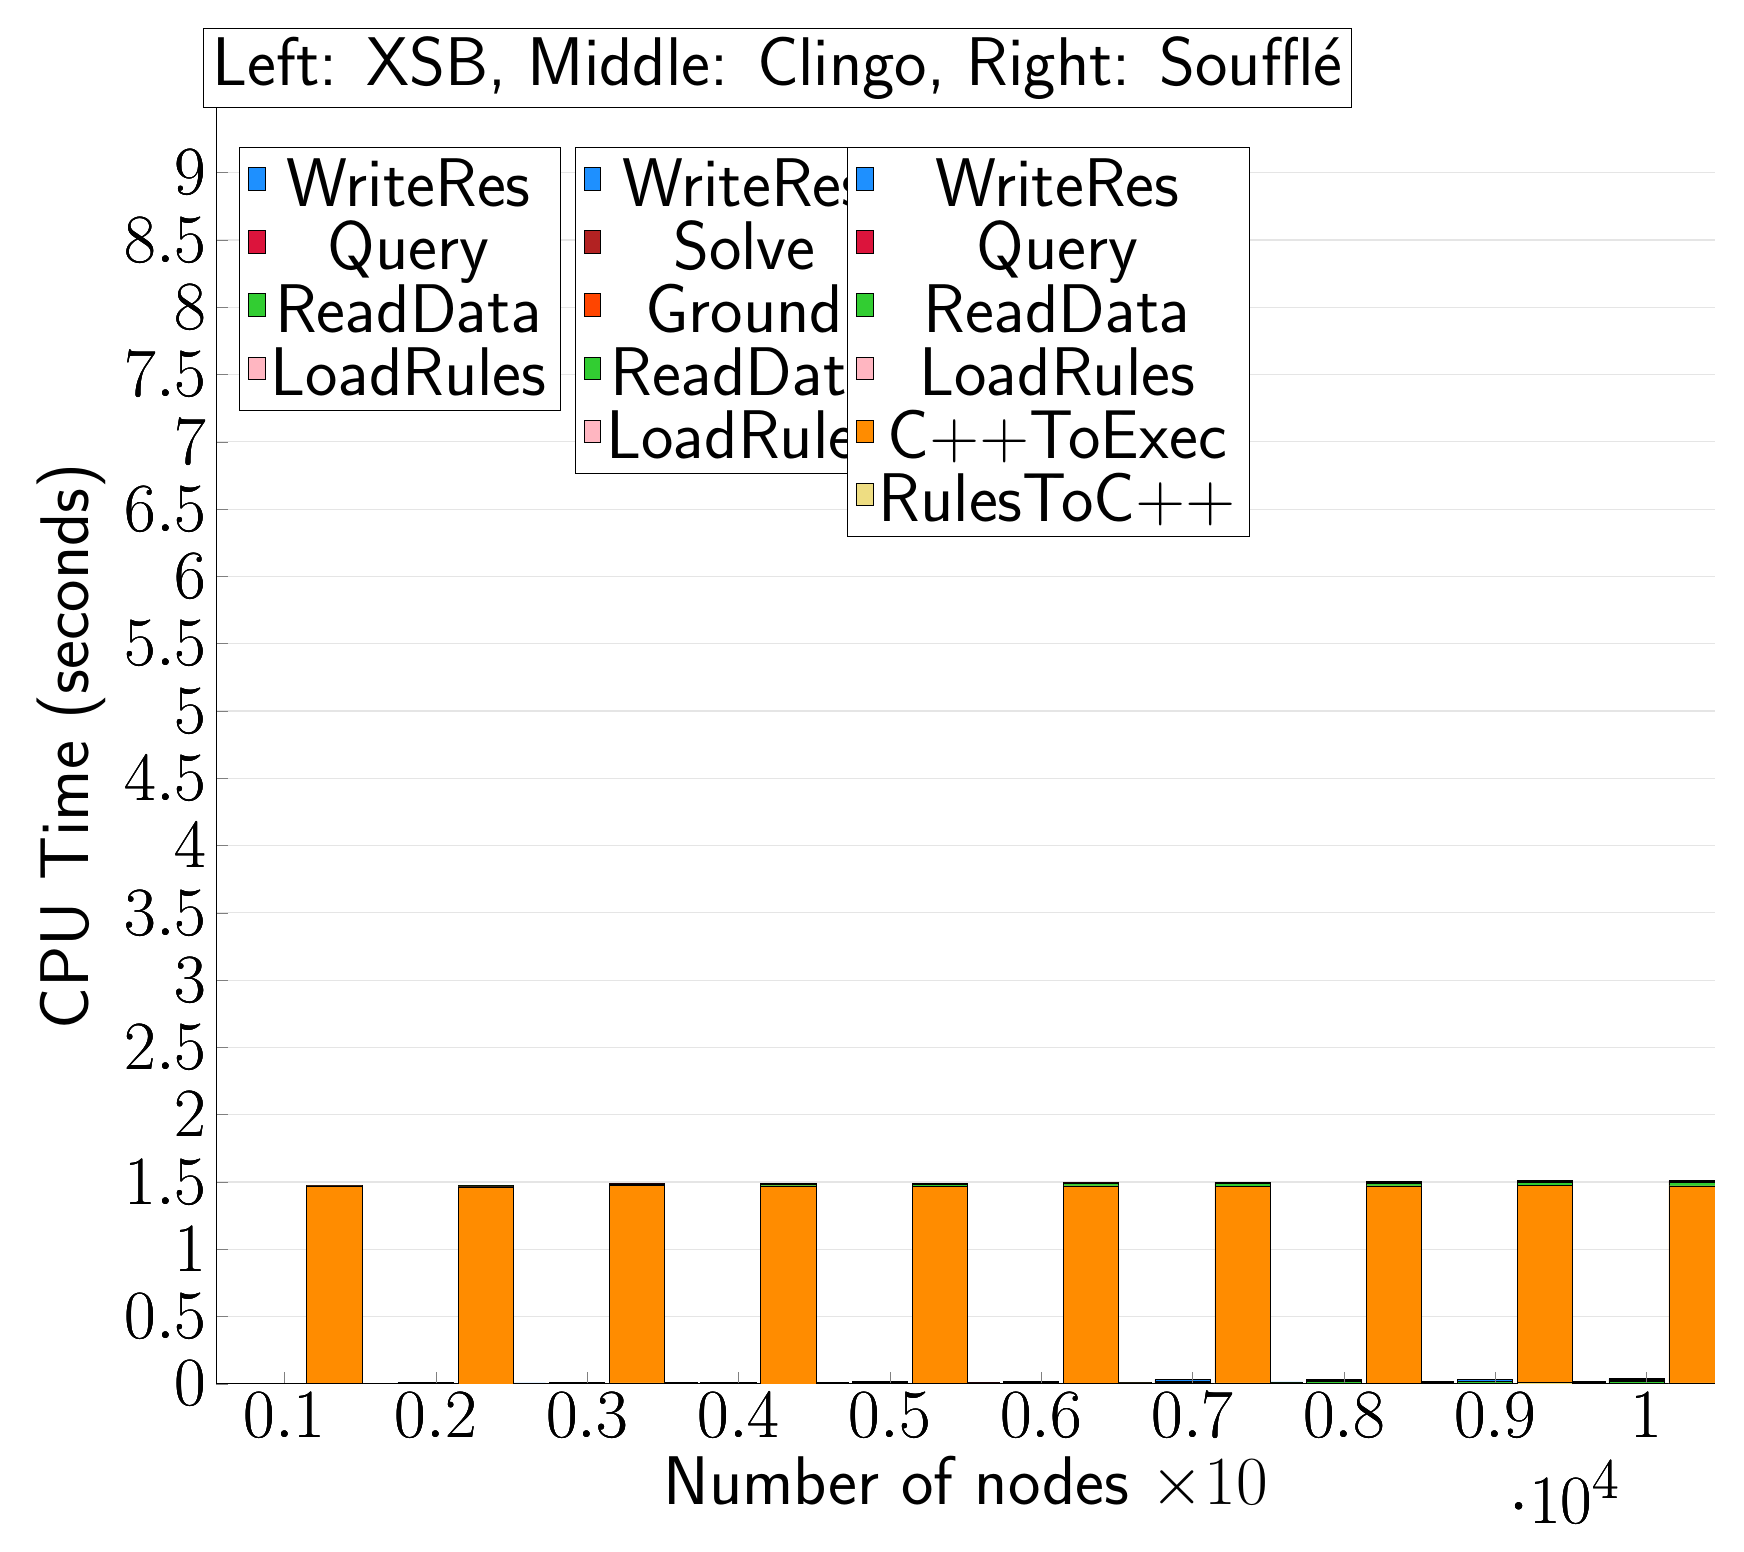
\begin{tikzpicture}
                        \begin{axis}[bar shift=-25pt, 
   ybar stacked,
   width=1.7\textwidth,
   bar width=0.7cm,
   ymajorgrids, tick align=inside,
   major grid style={draw=gray!20},
   xtick=data,
   ymin=0, ymax=9.478,
   axis x line*=bottom,
   axis y line*=left,
   enlarge x limits=0.05,
   legend style={
       at={(0.23, 0.97)},
       anchor=north east,
       legend columns=1,
       font=\Huge,
   },
   ylabel={CPU Time (seconds)},
   xlabel={Number of nodes $\times 10$},
   label style={font=\Huge},
   tick label style={font=\Huge},
]
\addlegendimage{fill=DodgerBlue, draw=black, line width=0.2pt}
\addlegendentry{WriteRes}
\addlegendimage{fill=Crimson, draw=black, line width=0.2pt}
\addlegendentry{Query}
\addlegendimage{fill=LimeGreen, draw=black, line width=0.2pt}
\addlegendentry{ReadData}
\addlegendimage{fill=LightPink, draw=black, line width=0.2pt}
\addlegendentry{LoadRules}
\addplot +[fill=LightPink, draw=black, line width=0.2pt] coordinates {
(1000, 0.0005499999999999995)
(2000, 0.0005474000000000002)
(3000, 0.0005481999999999993)
(4000, 0.0005488000000000004)
(5000, 0.0005486000000000005)
(6000, 0.0005487999999999995)
(7000, 0.0005485999999999996)
(8000, 0.0005502)
(9000, 0.0005513999999999996)
(10000, 0.0005487999999999998)
};
\addplot +[fill=LimeGreen, draw=black, line width=0.2pt] coordinates {
(1000, 0.0008966000000000003)
(2000, 0.001687)
(3000, 0.0024723999999999996)
(4000, 0.0032554)
(5000, 0.0040406)
(6000, 0.0048918)
(7000, 0.0057155999999999995)
(8000, 0.0065224)
(9000, 0.007375200000000001)
(10000, 0.008212)
};
\addplot +[fill=Crimson, draw=black, line width=0.2pt] coordinates {
(1000, 0.0001273999999999996)
(2000, 0.000248199999999999)
(3000, 0.000389199999999999)
(4000, 0.0005428000000000002)
(5000, 0.0006617999999999992)
(6000, 0.0007769999999999996)
(7000, 0.000909999999999999)
(8000, 0.001036)
(9000, 0.0011784)
(10000, 0.0013002)
};
\addplot +[fill=DodgerBlue, draw=black, line width=0.2pt] coordinates {
(1000, 0.0009104000000000004)
(2000, 0.0017386000000000012)
(3000, 0.002579800000000001)
(4000, 0.0034097999999999997)
(5000, 0.004271800000000001)
(6000, 0.0050760000000000015)
(7000, 0.005926000000000001)
(8000, 0.0068195999999999994)
(9000, 0.0076888)
(10000, 0.0083894)
};
\end{axis}

\begin{axis}[bar shift=-3.7pt, 
   ybar stacked,
   width=1.7\textwidth,
   bar width=0.7cm,
   ymajorgrids, tick align=inside,
   major grid style={draw=none},
   xtick=data,
   ymin=0, ymax=9.478,
   axis x line*=none,
   axis y line*=none,
   enlarge x limits=0.05,
   legend style={
       at={(0.454, 0.97)},
       anchor=north east,
       legend columns=1,
       font=\Huge,
   },
   label style={font=\Huge},
   tick label style={font=\Huge},
]
\addlegendimage{fill=DodgerBlue, draw=black, line width=0.2pt}
\addlegendentry{WriteRes}
\addlegendimage{fill=FireBrick, draw=black, line width=0.2pt}
\addlegendentry{Solve}
\addlegendimage{fill=OrangeRed, draw=black, line width=0.2pt}
\addlegendentry{Ground}
\addlegendimage{fill=LimeGreen, draw=black, line width=0.2pt}
\addlegendentry{ReadData}
\addlegendimage{fill=LightPink, draw=black, line width=0.2pt}
\addlegendentry{LoadRules}
\addplot +[fill=LightPink, draw=black, line width=0.2pt] coordinates {
(1000, 0.0)
(2000, 0.0)
(3000, 0.0)
(4000, 0.0)
(5000, 0.0)
(6000, 0.0)
(7000, 0.0)
(8000, 0.0)
(9000, 0.0)
(10000, 0.0)
};
\addplot +[fill=LimeGreen, draw=black, line width=0.2pt] coordinates {
(1000, 0.0)
(2000, 0.0)
(3000, 0.0)
(4000, 0.010000000000000009)
(5000, 0.010000000000000009)
(6000, 0.010000000000000009)
(7000, 0.010000000000000009)
(8000, 0.018000000000000016)
(9000, 0.020000000000000018)
(10000, 0.020000000000000018)
};
\addplot +[fill=OrangeRed, draw=black, line width=0.2pt] coordinates {
(1000, 0.0)
(2000, 0.0)
(3000, 0.010000000000000009)
(4000, 0.0)
(5000, 0.0)
(6000, 0.0020000000000000018)
(7000, 0.010000000000000009)
(8000, 0.006000000000000005)
(9000, 0.0)
(10000, 0.008000000000000007)
};
\addplot +[fill=FireBrick, draw=black, line width=0.2pt] coordinates {
(1000, 0.0)
(2000, 0.0)
(3000, 0.0)
(4000, 0.0)
(5000, 0.0)
(6000, 0.0040000000000000036)
(7000, 0.0)
(8000, 0.0)
(9000, 0.0)
(10000, 0.0020000000000000018)
};
\addplot +[fill=DodgerBlue, draw=black, line width=0.2pt] coordinates {
(1000, 0.0)
(2000, 0.010000000000000009)
(3000, 0.0)
(4000, 0.0)
(5000, 0.010000000000000009)
(6000, 0.0)
(7000, 0.010000000000000009)
(8000, 0.010000000000000009)
(9000, 0.010000000000000009)
(10000, 0.008000000000000007)
};
\end{axis}

\begin{axis}[bar shift=18pt, 
   ybar stacked,
   width=1.7\textwidth,
   bar width=0.7cm,
   ymajorgrids, tick align=inside,
   major grid style={draw=none},
   xtick=data,
   ymin=0, ymax=9.478,
   axis x line*=none,
   axis y line*=none,
   enlarge x limits=0.05,
   legend style={
       at={(0.69, 0.97)},
       anchor=north east,
       legend columns=1,
       font=\Huge,
   },
   label style={font=\Huge},
   tick label style={font=\Huge},
]
\addlegendimage{fill=DodgerBlue, draw=black, line width=0.2pt}
\addlegendentry{WriteRes}
\addlegendimage{fill=Crimson, draw=black, line width=0.2pt}
\addlegendentry{Query}
\addlegendimage{fill=LimeGreen, draw=black, line width=0.2pt}
\addlegendentry{ReadData}
\addlegendimage{fill=LightPink, draw=black, line width=0.2pt}
\addlegendentry{LoadRules}
\addlegendimage{fill=DarkOrange, draw=black, line width=0.2pt}
\addlegendentry{C++ToExec}
\addlegendimage{fill=LightGoldenrod, draw=black, line width=0.2pt}
\addlegendentry{RulesToC++}
\addplot +[fill=LightGoldenrod, draw=black, line width=0.2pt] coordinates {
(1000, 0.0020000000000000005)
(2000, 0.0)
(3000, 0.006000000000000001)
(4000, 0.0)
(5000, 0.004000000000000001)
(6000, 0.004000000000000001)
(7000, 0.006000000000000001)
(8000, 0.0020000000000000005)
(9000, 0.008000000000000002)
(10000, 0.006000000000000001)
};
\addplot +[fill=DarkOrange, draw=black, line width=0.2pt] coordinates {
(1000, 1.468)
(2000, 1.464)
(3000, 1.466)
(4000, 1.47)
(5000, 1.464)
(6000, 1.4659999999999997)
(7000, 1.462)
(8000, 1.468)
(9000, 1.466)
(10000, 1.464)
};
\addplot +[fill=LightPink, draw=black, line width=0.2pt] coordinates {
(1000, 0.0001538)
(2000, 0.00014359999999999997)
(3000, 0.0001608)
(4000, 0.0001548)
(5000, 0.00015979999999999998)
(6000, 0.00015020000000000002)
(7000, 0.0001656)
(8000, 0.000157)
(9000, 0.00015)
(10000, 0.0001518)
};
\addplot +[fill=LimeGreen, draw=black, line width=0.2pt] coordinates {
(1000, 0.0036458)
(2000, 0.006354)
(3000, 0.0095072)
(4000, 0.012687799999999999)
(5000, 0.014790399999999999)
(6000, 0.0164132)
(7000, 0.0193182)
(8000, 0.020308)
(9000, 0.023471400000000003)
(10000, 0.025407000000000002)
};
\addplot +[fill=Crimson, draw=black, line width=0.2pt] coordinates {
(1000, 0.0014572)
(2000, 0.0025206)
(3000, 0.004229)
(4000, 0.004694)
(5000, 0.006256599999999999)
(6000, 0.007191400000000001)
(7000, 0.0084206)
(8000, 0.0087794)
(9000, 0.0094808)
(10000, 0.010449799999999999)
};
\addplot +[fill=DodgerBlue, draw=black, line width=0.2pt] coordinates {
(1000, 0.0008618)
(2000, 0.0010382)
(3000, 0.0017202000000000003)
(4000, 0.0020222)
(5000, 0.00229)
(6000, 0.0025908000000000003)
(7000, 0.0028786000000000003)
(8000, 0.0029268)
(9000, 0.0032782000000000006)
(10000, 0.0033824)
};
\end{axis}


\node[anchor=south, draw, fill=white] at (rel axis cs:0.42,1) {\Huge Left: XSB, Middle: Clingo, Right: Soufflé};
\end{tikzpicture}
\end{document}
                    